
\documentclass[12pt, a4paper]{article}

\usepackage[ruled, vlined]{algorithm2e}
\usepackage{rotating}
\usepackage{graphics}

\author{Hong Lu \\ luh.lewis@gmail.com}
\date{}

\begin{document}
    \title{Is task clustering executable}
    \maketitle

    \section{Reviews}
    \subsection*{How to deal with the tasks?}
    We can adapt several representations to the tasks by using various algorithms based on different data structures.
    The idea, we often bring about easily, is to connect or divide the tasks into an entity or several groups.
    \subsubsection*{k-means}
    Within clustering algorithm, k-means is efficient and gurantees to converge. 
    
    It depends that what constitutes good clusters subjecting to various criteria, both ad-hoc or systematic.  
    
    Some experiments are shown below in Fig.~\ref{fig:random k-means}

    \begin{sidewaysfigure}
        \centering
        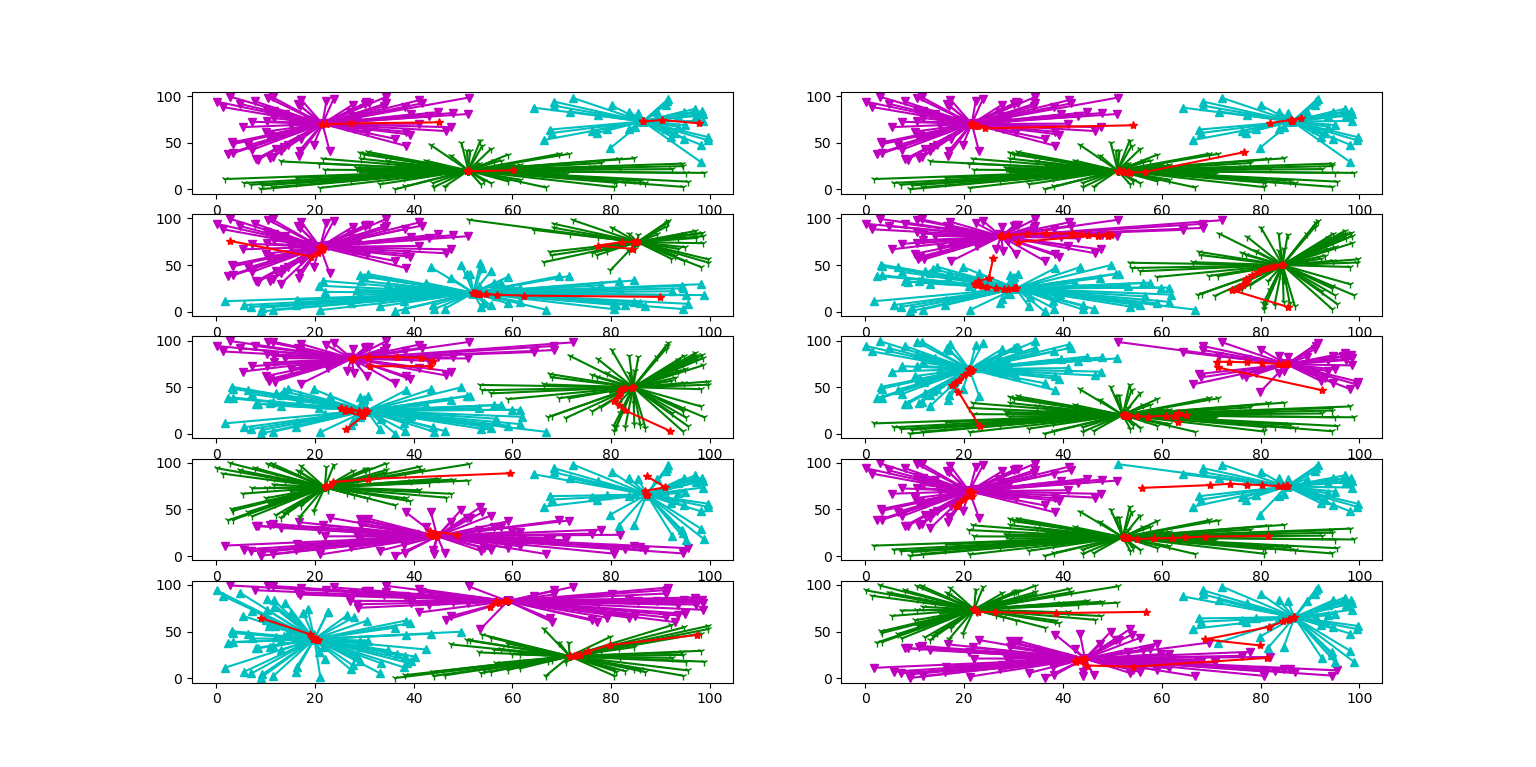
\includegraphics[width = 1.3\textwidth]{../img/randomcentroid.png}
        \caption{random initial centroid}
        \label{fig:random k-means}
    \end{sidewaysfigure}

    simple k-means is shown as algorithm~\ref{simple k-means}
    
    \subsubsection*{Yinyang k-means}
    Yinyang k-means, proposed @ICML in 2015, optimizes $Assignment$ process of algorithm~\ref{simple k-means} mainly.
    It uses Triangle inequality to reduce computations which has been implemented before.
    Let's introduce some notations, $c_{i} \in C,\; i = 1,2,3,...,k$, where $C$ represents set of cluster centers and $c$ is a cluster within the set.
    Let $b(x)$ ("the best cluster for") be the cluster to which the point is assigned to. Let $b'(x), c',C'$ be the entity in the next iteration.
    Let $\sigma(c)$ represents $d(c, c')$

    Global filtering identifies whether a point $x$ changes its cluster in an assignment step with a \textbf{single} comparison.
    Algorithm maintains an upper and lower bound, where $ub(x) \geq d(x, b(x))$ and $lb(x) \leq d(x,c), \forall c \in C-b(x)$


    \begin{algorithm}[H]
        \SetAlgoLined
        \DontPrintSemicolon

        \KwData{k, Points, initial centroids}  
        \KwResult{Clusters: C}
        \Begin{
        Initialization\;\Begin{
            $centroids \gets \textnormal{initial centroids}$\\
            C, result = $\textbf{Assginment}$($points$, $centroids$)\\
        }            
        \While{result not converges}{
            $centroids$ = $\textbf{Update Centroid}(C)$\\       
            C, result = $\textbf{Assginment}$($points$, $centroids$)\\
            \If{Assginment not change}{
                result converges
            }
        }
        \Return{C}\\
        }
        \;
        $\textbf{Update Centroid}($Clusters$)$\\
        \Begin{
            \For{$C_{i}$ in Clusters}{
                \For{$p_{j}$ in $C_{i}$}{
                    $centroid_{i} = \frac{1}{M}\sum{p_{j}}$
                }
            }
            \Return{centroids}
        }
        \;
        $\textbf{Assignment}($points$, $centroids$)$\\
        \Begin{
            \For{$p$ in $Points$}{
                Calculate Distance between $p$ and $centroids_{i}, \; i = 1, 2, 3,...,k$\\
                Store Nearest centroid $c^{*}$ of $p$
            }
            assign $p_{i}$ to respective $c_{i}^*$ in $C$
            \If{assignment is stable}{
               \Return{C, converge}
            }
            \Return{C, not converge}
        }

        \caption{Jejune K-means: Centroid-based k-means}
        \label{simple k-means}
    \end{algorithm}
\end{document}